\documentclass[unknownkeysallowed]{beamer}
\usepackage[french,english]{babel}
\usepackage{./tex/sty/beamer_js}
\usepackage{./tex/sty/shortcuts_js}
\usepackage{etex}
\usepackage{csquotes}
\usepackage{stmaryrd}


\newcommand*{\AIC}{\mathrm{AIC}}
\newcommand*{\BIC}{\mathrm{BIC}}

\addbibresource{bibli.bib}



\begin{document}


%%%%%%%%%%%%%%%%%%%%%%%%%%%%%%%%%%%%%%%%%%%%%%%%%%%%%%%%%%%%%%%%%%%%%%%%%%%%%%%
%%%%%%%%%%%%%%%%%%%%%%             Headers               %%%%%%%%%%%%%%%%%%%%%%
%%%%%%%%%%%%%%%%%%%%%%%%%%%%%%%%%%%%%%%%%%%%%%%%%%%%%%%%%%%%%%%%%%%%%%%%%%%%%%%



%%%%%%%%%%%%%%%%%%%%%%%%%%%%%%%%%%%%%%%%%%%%%%%%%%%%%%%%%%%%%%%%%%%%%%%%%%%%%%%
\begin{frame}
\bigskip
\bigskip
\begin{center}{
\LARGE\color{marron}
\textbf{HMMA307 - Project}
\textbf{ }\\
\vspace{0.5cm}
}

\color{marron}
\textbf{Linear mixed models}
\end{center}

\vspace{0.5cm}

\begin{center}
\textbf{Fanchon Herman} \\
\vspace{0.1cm}
\url{https://github.com/fanchonherman/HMMA307-Project}\\
\vspace{0.5cm}
Université de Montpellier \\
\end{center}

\centering

\includegraphics[width=0.13\textwidth]{./images/Logo}

\end{frame}
%%%%%%%%%%%%%%%%%%%%%%%%%%%%%%%%%%%%%%%%%%%%%%%%%%%%%%%%%%%%%%%%%%%%%%%%%%%%%%%


%%%%%%%%%%%%%%%%%%%%%%%%%%%%%%%%%%%%%%%%%%%%%%%%%%%%%%%%%%%%%%%%%%%%%%%%%%%%%%%
%%%%%%%%%%%%%%%%%%%%%%%%       PLAN      %%%%%%%%%%%%%%%%%%%%%%%%%%%%%%%%%%%%%%
%%%%%%%%%%%%%%%%%%%%%%%%%%%%%%%%%%%%%%%%%%%%%%%%%%%%%%%%%%%%%%%%%%%%%%%%%%%%%%%



%%%%%%%%%%%%%%%%%%%%%%%%%%%%%%%%%%%%%%%%%%%%%%%%%%%%%%%%%%%%%%%%%%%%%%%%%%%%%%%
\begin{frame}{Table of Contents}
\tableofcontents[hideallsubsections]
\end{frame}
%%%%%%%%%%%%%%%%%%%%%%%%%%%%%%%%%%%%%%%%%%%%%%%%%%%%%%%%%%%%%%%%%%%%%%%%%%%%%%%

%%%%%%%%%%%%%%%%%%%%%%%%%%%%%%%%%%%%%%%%%%%%%%%%%%%%%%%%%%%%%%%%%%%%%%%%%%%%%%%
%\AtBeginSection[]
%{
%\begin{frame}<beamer>{Table of Contents}
%\tableofcontents[currentsubsection,
%    hideothersubsections,
%    sectionstyle=show/shaded,
%]
%\end{frame}
%}
%%%%%%%%%%%%%%%%%%%%%%%%%%%%%%%%%%%%%%%%%%%%%%%%%%%%%%%%%%%%%%%%%%%%%%%%%%%%%%%

%%%%%%%%%%%%%%%%%%%%%%%%%%%%%%%%%%%%%%%%%%%%%%%%%%%%%%%%%%%%%%%%%%%%%%%%%%%%%%%
%%%%%%%%%%%%%%%%%%%%%%%%%%%%%%%%%%%%%%%%%%%%%%%%%%%%%%%%%%%%%%%%%%%%%%%%%%%%%%%
\section{Introduction}
\label{sec:introdcution}
%%%%%%%%%%%%%%%%%%%%%%%%%%%%%%%%%%%%%%%%%%%%%%%%%%%%%%%%%%%%%%%%%%%%%%%%%%%%%%
%%%%%%%%%%%%%%%%%%%%%%%%%%%%%%%%%%%%%%%%%%%%%%%%%%%%%%%%%%%%%%%%%%%%%%%%%%%%%%%

%%%%%%%%%%%%%%%%%%%%%%%%%%%%%%%%%%%%%%%%%%%%%%%%%%%%%%%%%%%%%%%%%%%%%%%%%%%%%%%
\begin{frame}{Introduction}
Linear mixed models :
\begin{itemize}
    \item Extension of simple linear models to have fixed and random effects,
    \item fixed effect: constant parameter,
    \item random effect: parameter that is random variable,
    \item used when the data is not independent.
    \end{itemize}
\end{frame}
%%%%%%%%%%%%%%%%%%%%%%%%%%%%%%%%%%%%%%%%%%%%%%%%%%%%%%%%%%%%%%%%%%%%%%%%%%%%%%%%

%%%%%%%%%%%%%%%%%%%%%%%%%%%%%%%%%%%%%%%%%%%%%%%%%%%%%%%%%%%%%%%%%%%%%%%%%%%%%%%
\begin{frame}{Data presentation}
\begin{itemize}
    \item From Grodner and Gibson, Expt $1$,
    \item analysis of the reading times at the relative clause verb in a self-paced reading study,
    \item $672$ observations, $42$ subjects and $4$ features.
\end{itemize}
\begin{center}
    \begin{tabular}{|c|c|c|c|c|c|}
    \hline
         subject & item & condition & rawRT & so & logrt  \\
         \hline \hline
         1 & 1 & objgap & 320 & 1 & 5.768\\
         42 & 16 & subjgap & 316 & -1 & 5.756\\
         \hline
    \end{tabular}
    \captionof{table}{Example of a data extract} 
\end{center}
\begin{itemize}
    \item feature so: represents the contrast coding,
    \item feature logrt: represents log-transformed reading time
\end{itemize}
\end{frame}
%%%%%%%%%%%%%%%%%%%%%%%%%%%%%%%%%%%%%%%%%%%%%%%%%%%%%%%%%%%%%%%%%%%%%%%%%%%%%%%%

%%%%%%%%%%%%%%%%%%%%%%%%%%%%%%%%%%%%%%%%%%%%%%%%%%%%%%%%%%%%%%%%%%%%%%%%%%%%%%%
%%%%%%%%%%%%%%%%%%%%%%%%%%%%%%%%%%%%%%%%%%%%%%%%%%%%%%%%%%%%%%%%%%%%%%%%%%%%%%%
\section{Model type 1: Varying intercepts}
%%%%%%%%%%%%%%%%%%%%%%%%%%%%%%%%%%%%%%%%%%%%%%%%%%%%%%%%%%%%%%%%%%%%%%%%%%%%%%
%%%%%%%%%%%%%%%%%%%%%%%%%%%%%%%%%%%%%%%%%%%%%%%%%%%%%%%%%%%%%%%%%%%%%%%%%%%%%%%

%%%%%%%%%%%%%%%%%%%%%%%%%%%%%%%%%%%%%%%%%%%%%%%%%%%%%%%%%%%%%%%%%%%%%%%%%%%%%%%
\begin{frame}{Equation of the model 1}
\mytheorem{Model equation}
{\[y_{ij}=\beta_0+ u_{0i} + \beta_1 \times so_{ij}+\varepsilon_{ij},\]}

\medskip

 \begin{itemize}
        \item By-subject adjustment to the intercept,
        \item $i \in \llbracket1,42\rrbracket$ indexes subjects, $j \in \llbracket1,16 \rrbracket$ indexes items,
        \item intercept and slope: fixed effects and $u_0$: random effect,
        \item $2$ sources of variance:
        \end{itemize}
 $$u_{0} {\sim} \mathcal{N}(0, \sigma_{u0}>0) \text{ ,}\enspace 
 \varepsilon {\sim} \mathcal{N}(0,\sigma>0).$$

\end{frame}
%%%%%%%%%%%%%%%%%%%%%%%%%%%%%%%%%%%%%%%%%%%%%%%%%%%%%%%%%%%%%%%%%%%%%%%%%%%%%%%%

%%%%%%%%%%%%%%%%%%%%%%%%%%%%%%%%%%%%%%%%%%%%%%%%%%%%%%%%%%%%%%%%%%%%%%%%%%%%%%%%
\begin{frame}{Formulas for model selection}
\vspace{-0.7cm}
\[\textit{\underline{Goal}: minimize the value of the criteria.}\]

\medskip

\mytheorem{$\AIC$ and $\BIC$ criteria}
{ \[\AIC=(-2) \times \log(\text{likelihood}) + 2 \times (p+1),\]
\[\BIC=(-2) \times \log(\text{likelihood}) + (p+1) \times \log(n),\]
}

\medskip

\begin{itemize}
    \item $1$: estimated residual variance,
    \item $p$: all the other parameters estimate,
    \item $n$: number of observations.
\end{itemize}
\end{frame}
%%%%%%%%%%%%%%%%%%%%%%%%%%%%%%%%%%%%%%%%%%%%%%%%%%%%%%%%%%%%%%%%%%%%%%%%%%%%%%%%

%%%%%%%%%%%%%%%%%%%%%%%%%%%%%%%%%%%%%%%%%%%%%%%%%%%%%%%%%%%%%%%%%%%%%%%%%%%%%%%%
\begin{frame}[fragile]{Results of the linear mixed model}
\begin{itemize}
    \item Package Statsmodels from Python
\end{itemize}
\begin{lstlisting}
model_0=smf.mixedlm("logrt~so",data,groups=data['subject'])
model_0f=model_0.fit()
print(model_0.summary())
\end{lstlisting}

\begin{center}
    \begin{tabular}{|c|c|c|c|c|c|}
    \hline
         $\hat{\sigma}$ & $\hat{\sigma}_{u0}$ & $\text{IC}(95\%)(\text{so})$ & parameters & $\AIC$ & $\BIC$ \\
         \hline \hline
         0.382 & 0.316 & 0.033 0.091 & $3+1$ & 735.682 & 753.723 \\
         \hline
    \end{tabular}
    \captionof{table}{Results of the first model} 
\end{center}
$\longrightarrow$ intercept explains around $40\%$ of the variations,

$\longrightarrow$  at the $5\%$ threshold, the slope is significantly different from $0$.
\end{frame}
%%%%%%%%%%%%%%%%%%%%%%%%%%%%%%%%%%%%%%%%%%%%%%%%%%%%%%%%%%%%%%%%%%%%%%%%%%%%%%%%

%%%%%%%%%%%%%%%%%%%%%%%%%%%%%%%%%%%%%%%%%%%%%%%%%%%%%%%%%%%%%%%%%%%%%%%%%%%%%%%%
\begin{frame}{Intercept adjustements by subject}
\begin{figure}[H]
    \centering
    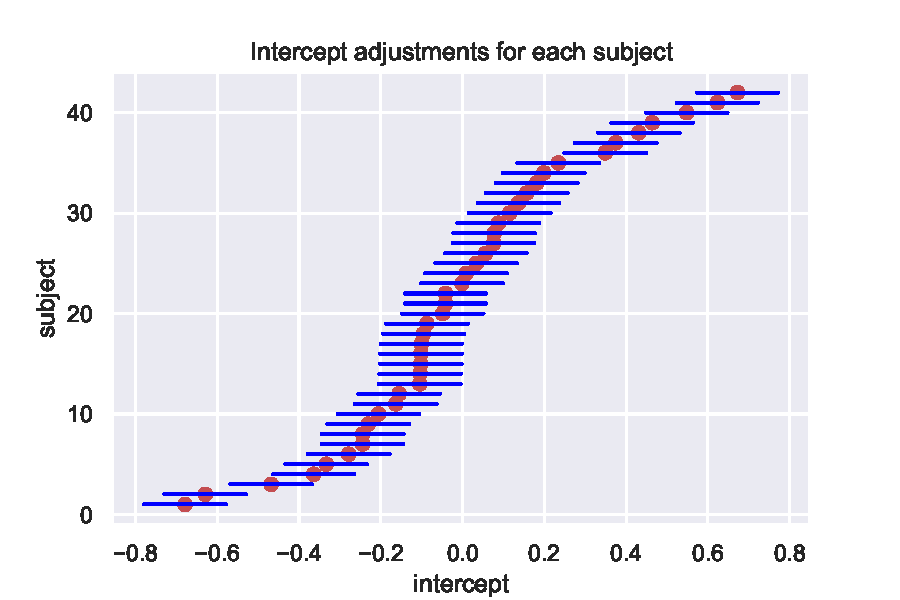
\includegraphics[scale=.45]{./images/model1_inter.pdf}
    \caption{Representation of the intercept adjustements by subject.}
\end{figure}
\vspace{-0.3cm}
\begin{align*}
    \longrightarrow \text{ }& 95\% \text{ confidence intervals},\\
    \longrightarrow \text{ }& \text{different intercept for each subject},\\
    \longrightarrow \text{ }& \text{large variability}.
\end{align*}
\end{frame}
%%%%%%%%%%%%%%%%%%%%%%%%%%%%%%%%%%%%%%%%%%%%%%%%%%%%%%%%%%%%%%%%%%%%%%%%%%%%%%%%


%%%%%%%%%%%%%%%%%%%%%%%%%%%%%%%%%%%%%%%%%%%%%%%%%%%%%%%%%%%%%%%%%%%%%%%%%%%%%%%
%%%%%%%%%%%%%%%%%%%%%%%%%%%%%%%%%%%%%%%%%%%%%%%%%%%%%%%%%%%%%%%%%%%%%%%%%%%%%%%
\section{Model type 2: Varying intercepts and slopes without correlation}
%%%%%%%%%%%%%%%%%%%%%%%%%%%%%%%%%%%%%%%%%%%%%%%%%%%%%%%%%%%%%%%%%%%%%%%%%%%%%%
%%%%%%%%%%%%%%%%%%%%%%%%%%%%%%%%%%%%%%%%%%%%%%%%%%%%%%%%%%%%%%%%%%%%%%%%%%%%%%%

%%%%%%%%%%%%%%%%%%%%%%%%%%%%%%%%%%%%%%%%%%%%%%%%%%%%%%%%%%%%%%%%%%%%%%%%%%%%%%%
\begin{frame}{Equation of the model 2}
\mytheorem{Model equation}
{\[y_{ij}=\beta_0+ u_{0i} + (\beta_1 + u_{1i})\times so_{ij}+\varepsilon_{ij}\]}

\medskip

 \begin{itemize}
        \item Without correlation,
        \item by-subject adjustment to the intercepts and slopes,
        \item $i \in \llbracket1,42\rrbracket$ indexes subjects, $j \in \llbracket1,16\rrbracket$ indexes items,
        \item $3$ sources of variance:
    \end{itemize}
$$u_{0} {\sim} \mathcal{N}(0, \sigma_{u0}>0) \text{ ,}\enspace u_{1} {\sim} \mathcal{N}(0, \sigma_{u1}>0)\enspace,$$
\vspace{-0.5cm}
$$\varepsilon {\sim} \mathcal{N}(0,\sigma>0).$$

\end{frame}
%%%%%%%%%%%%%%%%%%%%%%%%%%%%%%%%%%%%%%%%%%%%%%%%%%%%%%%%%%%%%%%%%%%%%%%%%%%%%%%%

%%%%%%%%%%%%%%%%%%%%%%%%%%%%%%%%%%%%%%%%%%%%%%%%%%%%%%%%%%%%%%%%%%%%%%%%%%%%%%%%
\begin{frame}{Results of the linear mixed model}
\begin{center}
    \begin{tabular}{|c|c|c|c|c|c|c|}
    \hline
         $\hat{\sigma}$ & $\hat{\sigma}_{u0}$ & $\hat{\sigma}_{u1}$ & $\text{IC}(95\%)(\text{so})$ & params & $\AIC$ & $\BIC$ \\
         \hline \hline
         0.366 & 0.317 & 0.110 & 0.019 0.105 & $4+1$ & 709.146 & 731.598 \\
         \hline
    \end{tabular}
    \captionof{table}{Results of the second model} 
\end{center}
$\longrightarrow$ intercept and adjusted slope explains around $50\%$ of the variations,
\newline
$\longrightarrow$  at the $5\%$ threshold, the slope is significantly different from $0$,
\newline
$\longrightarrow$ second model less "bad" than the first.
\end{frame}
%%%%%%%%%%%%%%%%%%%%%%%%%%%%%%%%%%%%%%%%%%%%%%%%%%%%%%%%%%%%%%%%%%%%%%%%%%%%%%%%

%%%%%%%%%%%%%%%%%%%%%%%%%%%%%%%%%%%%%%%%%%%%%%%%%%%%%%%%%%%%%%%%%%%%%%%%%%%%%%%%
\begin{frame}{Intercept and slope adjustements by subject}
    \begin{figure}[H]
    \centering
    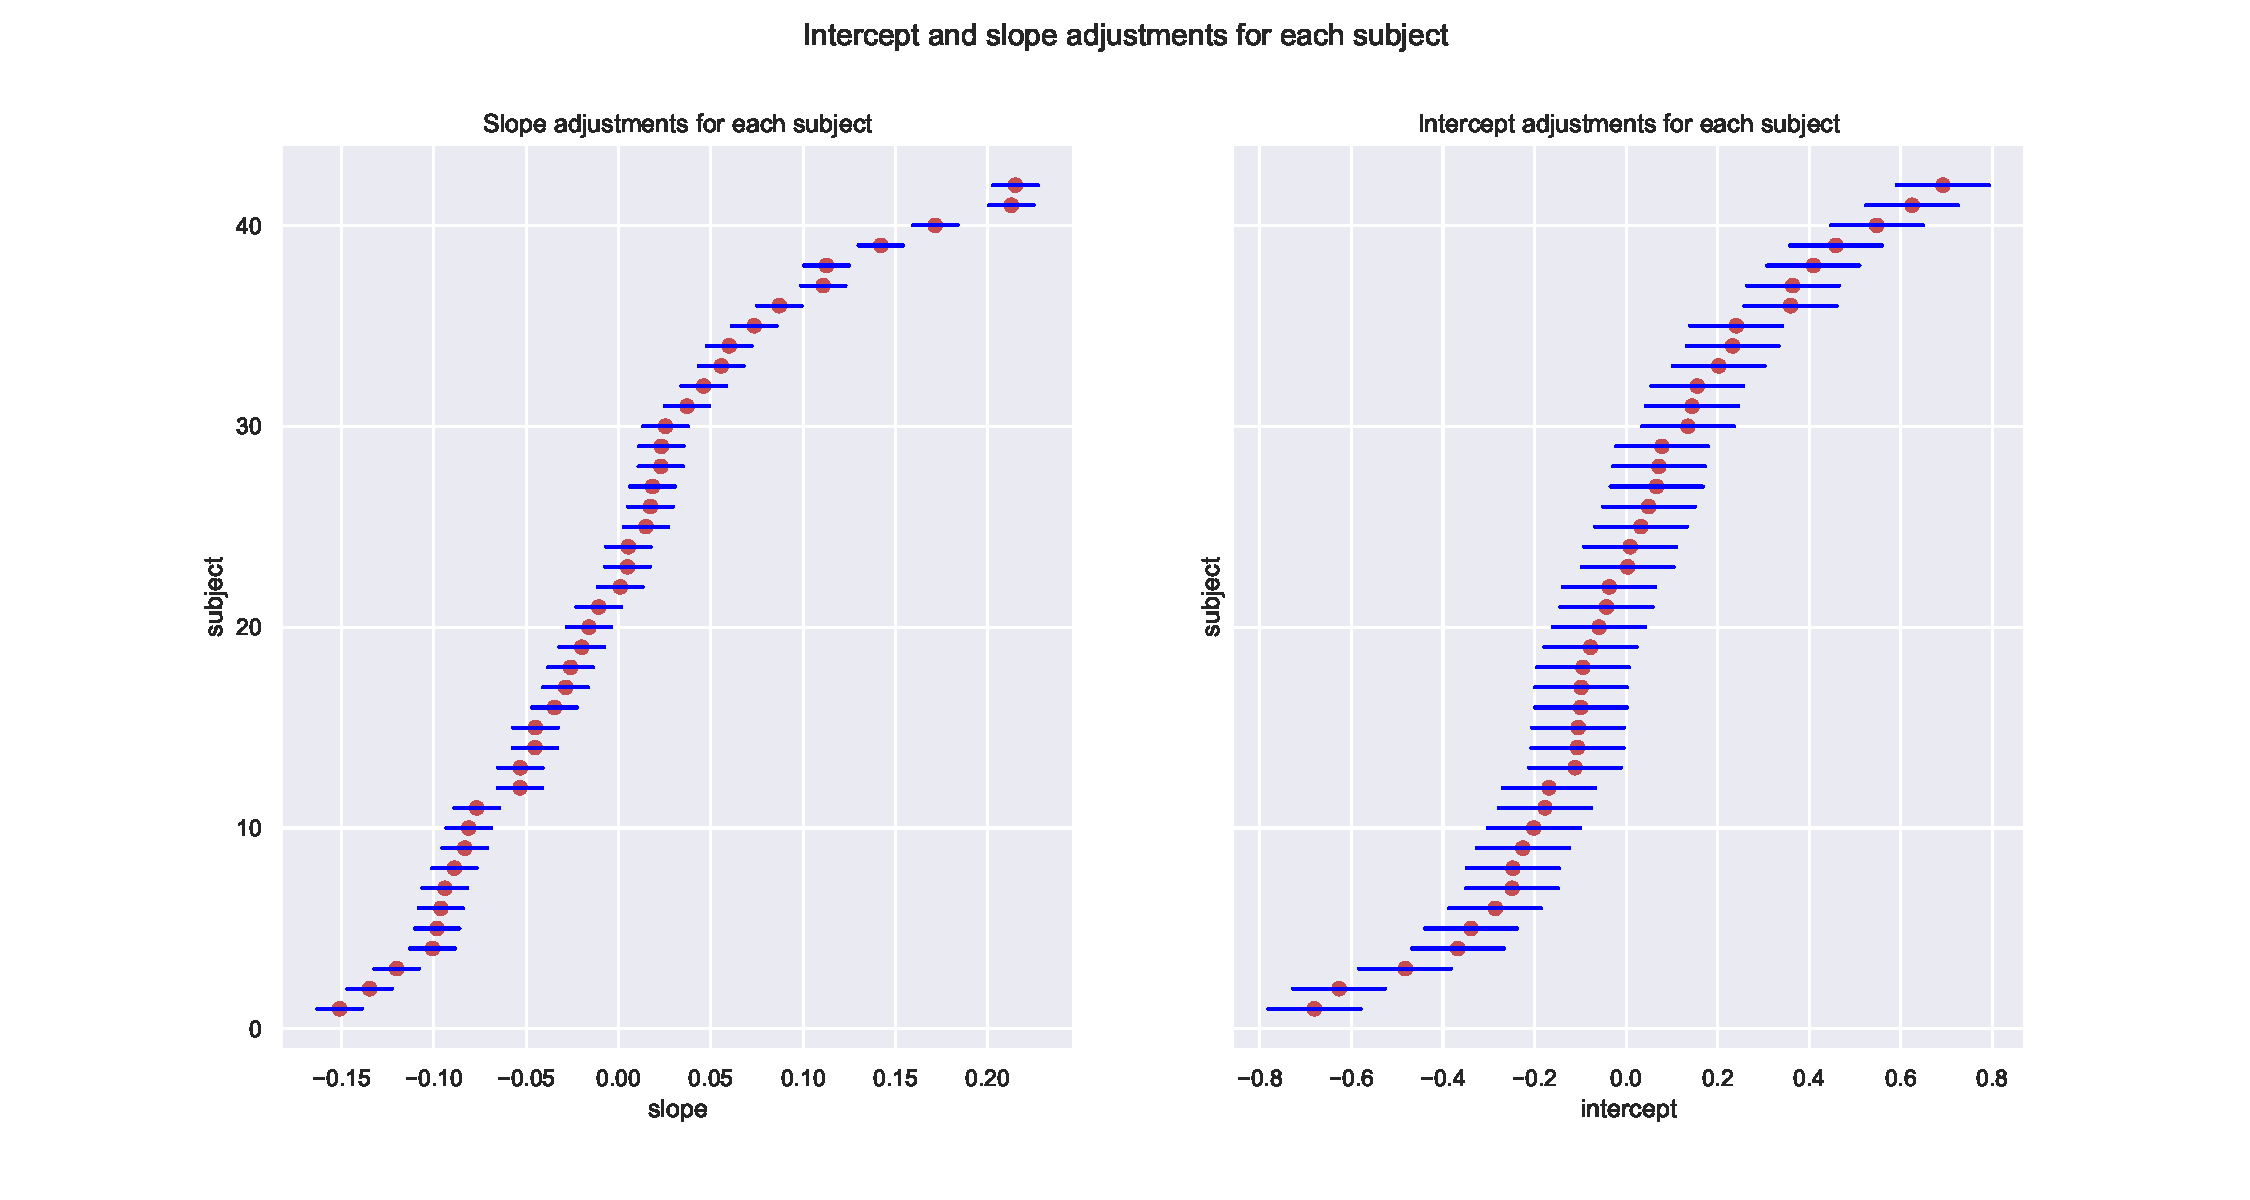
\includegraphics[scale=.24]{./images/model2_inter.pdf}
    \caption{Graphic of the intercept and slope adjustements by subject.}
    \end{figure}
\vspace{-0.3cm}
\begin{align*}
    \longrightarrow \text{ }& 95\% \text{ confidence intervals},\\
    \longrightarrow \text{ }& \text{different intercept for each subject},\\
    \longrightarrow \text{ }& \text{low variability in slope},\\
    \longrightarrow \text{ }& \text{large variability in intercept}.
\end{align*}
\end{frame}
%%%%%%%%%%%%%%%%%%%%%%%%%%%%%%%%%%%%%%%%%%%%%%%%%%%%%%%%%%%%%%%%%%%%%%%%%%%%%%%%

%%%%%%%%%%%%%%%%%%%%%%%%%%%%%%%%%%%%%%%%%%%%%%%%%%%%%%%%%%%%%%%%%%%%%%%%%%%%%%%%
\begin{frame}{Model validation}
\vspace{-0.7cm}
\[\textit{Check the homogeneity of residues}\]
\begin{figure}[H]
\centering
\begin{subfigure}{.5\textwidth}
  \centering
  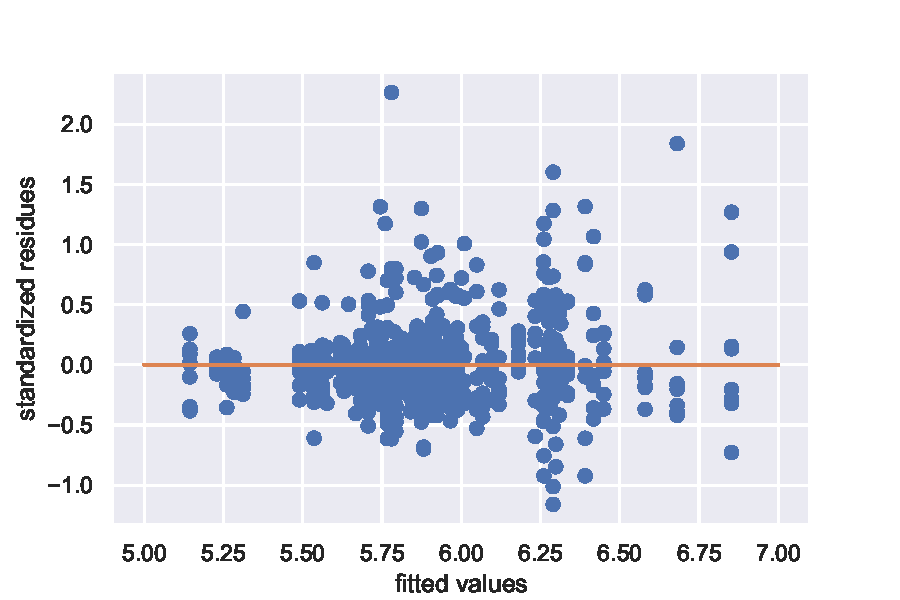
\includegraphics[width=1\linewidth]{./images/homo_mod2.pdf}
  \caption{Representation of the predicted by residual values.}
\end{subfigure}%
\begin{subfigure}{.5\textwidth}
  \centering
  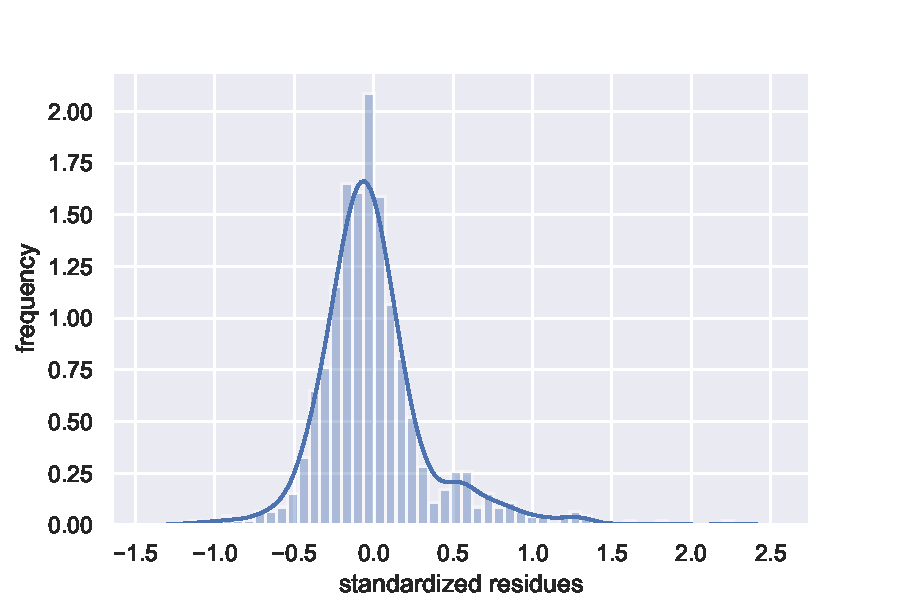
\includegraphics[width=1\linewidth, clip,trim={0cm 0cm 0cm 0cm} ]{./images/resid_norm_m2.pdf}
  \caption{Representation of the normality of the residuals.}
\end{subfigure}
\end{figure}
\begin{align*}
    \longrightarrow \text{ }& \text{residues: mainly close to the orange line},\\
    \longrightarrow \text{ }& \text{model fits our data well},\\
    \longrightarrow \text{ }& \text{normality of the residuals}.
\end{align*}
\end{frame}
%%%%%%%%%%%%%%%%%%%%%%%%%%%%%%%%%%%%%%%%%%%%%%%%%%%%%%%%%%%%%%%%%%%%%%%%%%%%%%%%

%%%%%%%%%%%%%%%%%%%%%%%%%%%%%%%%%%%%%%%%%%%%%%%%%%%%%%%%%%%%%%%%%%%%%%%%%%%%%%%
%%%%%%%%%%%%%%%%%%%%%%%%%%%%%%%%%%%%%%%%%%%%%%%%%%%%%%%%%%%%%%%%%%%%%%%%%%%%%%%
\section{Model type 3: Varying intercepts and slopes withe correlation}
%%%%%%%%%%%%%%%%%%%%%%%%%%%%%%%%%%%%%%%%%%%%%%%%%%%%%%%%%%%%%%%%%%%%%%%%%%%%%%
%%%%%%%%%%%%%%%%%%%%%%%%%%%%%%%%%%%%%%%%%%%%%%%%%%%%%%%%%%%%%%%%%%%%%%%%%%%%%%%

%%%%%%%%%%%%%%%%%%%%%%%%%%%%%%%%%%%%%%%%%%%%%%%%%%%%%%%%%%%%%%%%%%%%%%%%%%%%%%%
\begin{frame}{Equation of the model 3}
\mytheorem{Model equation}
{\[y_{ij}=\alpha + u_{0i} + w_{0j} + (\beta + u_{1i} + w_{1j})\times so_{ij}+\varepsilon_{ij}\]}

\medskip

 \begin{itemize}
        \item Correlation introduced,
        %between the intercept and slope adjustments,
        \item $i \in \llbracket1,42\rrbracket$ indexes subjects, $j \in \llbracket1,16\rrbracket$ indexes items,
        \item $\varepsilon \sim \mathcal{N}(0,\sigma>0),$
        \item $\begin{pmatrix}
        u_0 \\
        u_1 \\
        \end{pmatrix}$ $\sim \mathcal{N}\left(\begin{pmatrix}
        0 \\
        0 \\
        \end{pmatrix}, \Sigma_u\right) \text{ ; }$ $\begin{pmatrix}
        w_0 \\
        w_1 \\
        \end{pmatrix}$ $\sim \mathcal{N}\left(\begin{pmatrix}
        0 \\
        0 \\
        \end{pmatrix}, \Sigma_w\right)$
    \end{itemize}
\end{frame}
%%%%%%%%%%%%%%%%%%%%%%%%%%%%%%%%%%%%%%%%%%%%%%%%%%%%%%%%%%%%%%%%%%%%%%%%%%%%%%%%

%%%%%%%%%%%%%%%%%%%%%%%%%%%%%%%%%%%%%%%%%%%%%%%%%%%%%%%%%%%%%%%%%%%%%%%%%%%%%%%%
%\begin{frame}{Variance-covariance matrix}
%\begin{itemize}
%    \item the variance-covariance matrix for subjects is : 
%    $$\Sigma_u=
%    \begin{pmatrix}
%            \sigma_{u0}^2 & \rho_u\sigma_{u0}\sigma_{u1} \\
%            \rho_u\sigma_{u0}\sigma_{u1} & \sigma_{u1}^2 \\ 
%        \end{pmatrix}$$
%        \item the variance-covariance matrix for items is : 
%    $$\Sigma_w=
%    \begin{pmatrix}
%            \sigma_{u0}^2 & \rho_u\sigma_{u0}\sigma_{u1} \\
%            \rho_u\sigma_{u0}\sigma_{u1} & \sigma_{u1}^2 \\ 
%        \end{pmatrix}$$
%\end{itemize}
%\end{frame}
%%%%%%%%%%%%%%%%%%%%%%%%%%%%%%%%%%%%%%%%%%%%%%%%%%%%%%%%%%%%%%%%%%%%%%%%%%%%%%%

%%%%%%%%%%%%%%%%%%%%%%%%%%%%%%%%%%%%%%%%%%%%%%%%%%%%%%%%%%%%%%%%%%%%%%%%%%%%%%%
\begin{frame}{Results of the linear mixed model}
\begin{itemize}
    \item Number of estimated parameters: $8+1$,
    \item $\AIC$ and $\BIC$ respectively equal to $717.146$ and $757.739$,
    \item minimal $\AIC$ and $\BIC$ for the second model,
    \item perfect positive correlation between varying intercepts and slopes for items
\end{itemize}
\end{frame}
%%%%%%%%%%%%%%%%%%%%%%%%%%%%%%%%%%%%%%%%%%%%%%%%%%%%%%%%%%%%%%%%%%%%%%%%%%%%%%%

%%%%%%%%%%%%%%%%%%%%%%%%%%%%%%%%%%%%%%%%%%%%%%%%%%%%%%%%%%%%%%%%%%%%%%%%%%%%%%%%
\begin{frame}{Correlation between intercept and slope by subjects}
    \begin{figure}[H]
    \centering
    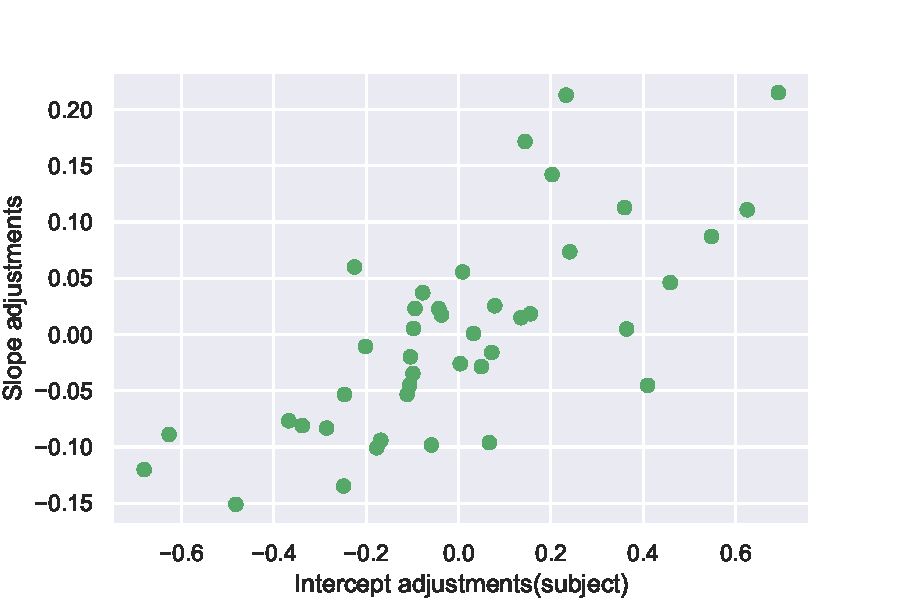
\includegraphics[scale=.45]{./images/adj_so_inter.pdf}
    \caption{Graphic of slope adjustements against intercept adjustements.}
    \end{figure}
\vspace{-0.3cm}
\begin{align*}
    \longrightarrow \text{ }&\text{data on the graph could fit a linear model},\\
    \longrightarrow \text{ }& \text{some noise on the data}.
\end{align*}
\end{frame}
%%%%%%%%%%%%%%%%%%%%%%%%%%%%%%%%%%%%%%%%%%%%%%%%%%%%%%%%%%%%%%%%%%%%%%%%%%%%%%%%

%%%%%%%%%%%%%%%%%%%%%%%%%%%%%%%%%%%%%%%%%%%%%%%%%%%%%%%%%%%%%%%%%%%%%%%%%%%%%%%%
\begin{frame}{Summary of the models}
\begin{center}
    \begin{tabular}{|c|c|c|c|c|c|}
    \hline
         & parameters & deviance & loglik & $\AIC$ & $\BIC$ \\
         \hline \hline
        model 1 & 4 & 727.682 & -363.841 & 735.682 & 753.723\\
        model 2 & 5 & 699.146 & -349.573 & 709.146 & 731.598\\
        model 3 & 9 & 699.146 & -349.573 &717.146 & 757.739\\
        \hline
    \end{tabular}
    \captionof{table}{Summary of the three models.} 
\end{center}
\end{frame}
%%%%%%%%%%%%%%%%%%%%%%%%%%%%%%%%%%%%%%%%%%%%%%%%%%%%%%%%%%%%%%%%%%%%%%%%%%%%%%%%

%%%%%%%%%%%%%%%%%%%%%%%%%%%%%%%%%%%%%%%%%%%%%%%%%%%%%%%%%%%%%%%%%%%%%%%%%%%%%%%
%%%%%%%%%%%%%%%%%%%%%%%%%%%%%%%%%%%%%%%%%%%%%%%%%%%%%%%%%%%%%%%%%%%%%%%%%%%%%%%
\section{Conclusion}
%%%%%%%%%%%%%%%%%%%%%%%%%%%%%%%%%%%%%%%%%%%%%%%%%%%%%%%%%%%%%%%%%%%%%%%%%%%%%%%
%%%%%%%%%%%%%%%%%%%%%%%%%%%%%%%%%%%%%%%%%%%%%%%%%%%%%%%%%%%%%%%%%%%%%%%%%%%%%%%

%%%%%%%%%%%%%%%%%%%%%%%%%%%%%%%%%%%%%%%%%%%%%%%%%%%%%%%%%%%%%%%%%%%%%%%%%%%%%%%
\begin{frame}{Conclusion}
\begin{itemize}
    \item Studied three different models,
    \item statistical model and validation for each, 
    \item least worse model for our data: second model.
\end{itemize}
\begin{figure}[H]
    \centering
    
\includegraphics[scale=.2]{./images/thanks.pdf}
    \end{figure}
\end{frame}
%%%%%%%%%%%%%%%%%%%%%%%%%%%%%%%%%%%%%%%%%%%%%%%%%%%%%%%%%%%%%%%%%%%%%%%%%%%%%%%%



%%%%%%%%%%%%%%%%%%%%%%%%%%%%%%%%%%%%%%%%%%%%%%%%%%%%%%%%%%%%%%%%%%%%%%%%%%%%%%%%
\begin{frame}{Bibliography}
\nocite{*}
\printbibliography
\end{frame}
 %%%%%%%%%%%%%%%%%%%%%%%%%%%%%%%%%%%%%%%%%%%%%%%%%%%%%%%%%%%%%%%%%%%%%%%%%%%%%%



\end{document}
